\chapter{{\bf Introduction}}
\label{sec:intro}


The Standard Model (SM)~\cite{GLASHOW1961579,PhysRevLett.19.1264,PhysRevD.2.1285} of particle physics is a Quantum Field Theory that describes the building blocks of matter and their interactions. It has been developed over several decades from a combination of theoretical progress and experimental discoveries. 
The SM predicts that all matter is constructed from combinations of particles called quarks or leptons and their anti-particles. The interactions between these particles are governed by the strong, weak and electromagnetic forces. 
There are a total of 6 quarks ({\it u, d, s, c, t, b}) and 6 anti-quarks ($\bar{u}$, $\bar{d}$, $\bar{s}$, $\bar{c}$, $\bar{b}$, $\bar{t}$) in the SM that can interact via all three forces. There are also 6 leptons ($e^{-}$, $\mu^{-}$, $\tau^{-}$, $\nu_e$, $\nu_{\mu}$, $\nu_{\tau}$) and 6 anti-leptons ($e^{+}$, $\mu^{+}$, $\tau^{+}$, $\overline{\nu}_e$, $\overline{\nu}_{\mu}$, $\overline{\nu}_{\tau}$), which, unlike quarks, leptons do interact via the strong force.
The interactions of each force are described by the exchange of gauge bosons. The electromagnetic force is mediated by the photon ($\gamma$), the weak force by the $W^{\pm}$ and $Z^0$ bosons and the strong force by eight gluons ($g$). 
The final particle in the SM is the Higgs boson ($H^0$). It is interactions with the field associated with this boson that are responsible for the intrinsic masses of the particles. The properties of the particles in the SM are given in Table~\ref{tab:fermions}.

\begin{table}[tbp]
\begin{center}
\begin{tabular}{lrrr}
\toprule
\toprule
Name & Symbol & Mass/\mevcc & Charge / $e$ \\ \midrule %& Spin \\ \midrule
Up & $u$ & $2.2^{+0.6}_{-0.4}$ & $\frac{2}{3}$ \\%& $\frac{1}{2}$ \\ 
Down & $d$ & $4.7^{+0.5}_{-0.4}$ & $-\frac{1}{3}$ \\%& $\frac{1}{2}$ \\
Charm & $c$ & $1270 \pm 30$& $\frac{2}{3}$ \\%& $\frac{1}{2}$ \\
Strange & $s$ &$96^{+8}_{-4}$ & $-\frac{1}{3}$ \\%& $\frac{1}{2}$ \\
Top & $t$ & $173210 \pm 510 \pm 710$ & $\frac{2}{3}$ \\%& $\frac{1}{2}$ \\
Bottom & $b$ & $4180^{40}_{30}$ & $-\frac{1}{3}$ \\%& $\frac{1}{2}$ \\
\midrule
Electron & $e^{-}$ & 0.5109989461 \pm 0.0000000031 & $-1$\\%& $\frac{1}{2}$ \\
Electron neutrino &$\nu_{e}$& $<0.000002$ & 0 \\%& 
Muon &$\mu^{-}$ & $105.6583745 \pm 0.0000024$  & $-1$ \\%& $\frac{1}{2}$ \\
Muon neutrino & $ \mu_{\mu}$& $<0.000002$ & 0 \\%&  
Tau &$\tau^{-}$& $1776.86 \pm 0.12$ & $-1$ \\ %& $\frac{1}{2}$ \\
Tau neutrino & $\nu_{\tau}$ & $<0.000002$ & 0 \\%&  
\midrule
Photon      & $\gamma$ & 0 & 0 \\
$W$ boson & $W^{\pm}$ & $80.385 \pm 0.015$ & $\pm1$ \\
$Z$ boson                      & $Z^{0}$ & $91.1876 \pm 0.0021$ & 0 \\
Gluons               & $g$ & 0 &  0\\
Higgs boson                   & $H^{0}$ & $125.09 \pm 0.21 \pm 0.11$ &0 \\ 
\bottomrule
\bottomrule
\end{tabular}
\vspace{0.7cm}
\caption{Mass and electric charge of particles in the SM taken from reference~\cite{Olive:2016xmw}. For quarks and lepton, only particles are listed; anti-particles have the same mass and opposite electric charge as their corresponding particles. All masses listed are measured values or limits except for the gluons and photon. In the SM the gluons and the photon do not couple to the Higgs field and are therefore massless. An upper limit has been placed on the photon mass at $1 \times 10^{-18}$~eV and gluon masses up to a few \mevcc are not excluded. The quark masses use the $\overline{\mathrm{MS}}$ renormalisation scheme and apart from the $t$ quark mass that comes from direct measurements.}
\label{tab:fermions}
\end{center}
\vspace{-1.0cm}
\end{table}



%\begin{table}[tbp]
%\begin{center}
%\begin{tabular}{llll}
%\toprule
%\toprule
%Name & Symbol & Mass/\mevcc & Charge / $e$ \\ \midrule %& Spin \\ \midrule                                                                                                                                  
%up quark & $u$ & $2.2^{+0.6}_{-0.4}$ & $\frac{2}{3}$ \\%& $\frac{1}{2}$ \\                                                                                                                                  
%down quark & $d$ & $4.7^{+0.5}_{-0.4}$ & $-\frac{1}{3}$ \\%& $\frac{1}{2}$ \\                                                                                                                               
%charm quark & $c$ & $1270 \pm 30$& $\frac{2}{3}$ \\%& $\frac{1}{2}$ \\                                                                                                                                      
%strange quark & $s$ &$96^{+8}_{-4}$ & $-\frac{1}{3}$ \\%& $\frac{1}{2}$ \\                                                                                                                                  
%top quark & $t$ & $173210 \pm 510 \pm 710$ & $\frac{2}{3}$ \\%& $\frac{1}{2}$ \\                                                                                                                            
%bottom quark & $b$ & $4180^{40}_{30}$ & $-\frac{1}{3}$ \\%& $\frac{1}{2}$ \\                                                                                                                                
%\midrule
%electron & $e^{-}$ & 0.5109989461 \pm 0.0000000031 & $-1$\\%& $\frac{1}{2}$ \\                                                                                                                              
%electron neutrino &$\nu_{e}$& $<0.000002$ & 0 \\%&                                                                                                                                                          
%muon &$\mu^{-}$ & $105.6583745 \pm 0.0000024$  & $-1$ \\%& $\frac{1}{2}$ \\                                                                                                                                 
%muon neutrino & $ \mu_{\mu}$& $<0.000002$ & 0 \\%&                                                                                                                                                          
%tau &$\tau^{-}$& $1776.86 \pm 0.12$ & $-1$ \\ %& $\frac{1}{2}$ \\                                                                                                                                           
%tau neutrino & $\nu_{\tau}$ & $<0.000002$ & 0 \\%&                                                                                                                                                          
%\bottomrule
%\bottomrule
%\end{tabular}
%\vspace{0.7cm}
%\caption{Measured mass and electric charge of quarks and leptons in the SM taken from reference~\cite{Olive:2016xmw}. Only particles are listed; anti-particles have the same mass and oposite electric cha\
%rge as their corresponding particles. The quark masses use the $\overline{\mathrm{MS}}$ renormalisation scheme and apart from the $t$ quark mass that comes from direct measurements.}
%\label{tab:fermions}
%\end{center}
%\vspace{-1.0cm}
%\end{table}%%

%\begin{table}[tbp]
%\begin{center}
%\begin{tabular}{llll}
%\toprule
%\toprule
%Force & Particle & Mass /\gevcc & Charge /$e$ \\ \midrule
%Electromagnetic       & $\gamma$ & 0 & 0 \\
%\multirow{2}{*}{Weak} & $W^{\pm}$ & $80.385 \pm 0.015$ & $\pm1$ \\
%                      & $Z^{0}$ & $91.1876 \pm 0.0021$ & 0 \\
%Strong                & $g$ & 0 &  0\\
% -                    & $H^{0}$ & $125.09 \pm 0.21 \pm 0.11$ 0 \\ 
%\bottomrule
%\bottomrule
%\end{tabular}
%\vspace{0.7cm}
%\caption{Mass and electric charge of gauge bosons and the Higgs boson. In the SM the gluons and the photon do not couple to the higgs field and are therefore massless. An upper limit has been placed on the photon mass at $1 \times 10^{-18}$~$e$V and gluon masses up to a few \mevcc are not excluded. Table values are taken from~\cite{Olive:2016xmw}.}
%\label{tab:bosons}
%\end{center}
%\vspace{-1.0cm}
%\end{table}%

The SM can be used to predict how particles will interact and decay. These predictions have been tested over the past decades and so far the SM has proved to be extremely successful. %no significant deviations from the predictions of the SM have been found. 
However, despite its success, there are a number of experimental observations that the SM does not explain. In its current form, the SM cannot explain the observed oscillation of neutrinos between different types~\cite{PhysRevLett.20.1205,Fukuda:1998fd, PhysRevLett.86.5656,PhysRevLett.87.071301} and it does not provide a particle or mechanism that could account for the observed presence of dark matter and dark energy in the universe~\cite{darkmatter1,darkmatter2,Dunkley:2008ie,Ade:2015xua}. 
The SM includes three fundamental forces but the final force, the gravitational force, is not included in its framework. 
Furthermore, at the start of the universe matter and anti-matter should have been produced in equal amounts but that is not what is observed in the universe today and the SM does not include a mechanism large enough to account for this asymmetry~\cite{Sakharov:1967dj,Gavela:1993ts}.
As well as experimental observations there are more fundamental questions about the SM that are unanswered. For example the SM does not explain why there are very large differences in the coupling strengths of the electromagnetic, weak and strong forces or why there is a large range in the masses of quarks and leptons.
The examples given here illustrate that despite the success of the SM it is not sufficient to describe the universe and indicate that it could be a low energy approximation of a more fundamental theory~\cite{lowenergySM}. A more complete discussion of the shortcomings of the SM can be found in references~\cite{Ellis:2002wba, Pomarol:2012sb}.

There exist many theories that go beyond the scope of the SM and seek to explain what the SM cannot. These theories predict the presence of new particles and phenomena that are collectively called New Physics (NP). At the moment there is no clear indication of which Beyond the SM (BSM) theory may give the correct description of the universe and the search for NP is ongoing.
The Large Hadron Collider (LHC) is the latest machine built to study the predictions of the SM and to search for NP in high energy particle collisions. There are two different approaches used to search for NP effects at the LHC and other experiments; direct searches and indirect searches.




Direct searches involve looking for the production of on-shell NP particles and phenomena in high energy collisions. 
This type of search is limited by the centre-of-mass energy of the collisions that dictates the energy available for the creation of new particles. 
The Higgs boson was discovered in 2012 by the ATLAS and CMS collaborations using this type of search~\cite{Chatrchyan:2012xdj,Aad:2012tfa} but no NP has been observed from direct searches to date. The lack of observations enables constraints to be placed on the parameter space of BSM theories.


Indirect searches precisely measure SM processes and look for deviations in the measured values from the predicted values. Deviations can be caused by the presence of NP that modifies the SM process. 
Indirect searches are not as limited by the centre-of-mass energy as direct searches because NP or SM particles influencing these processes are off-shell. % and therefore lower energy is needed to produce them. 
In a similar way to direct searches, indirect searches that do not reveal NP place constraints on the parameter space of the theoretical models. Although indirect searches are yet to reveal any significant deviations from SM predictions, some interesting anomalies have been seen in measured results in heavy flavour physics. 
In $b \to sll$ transitions, where $\ell = e, \mu$,  deviations from the SM predictions have been seen in measurements of the angular distribution of $B^0 \to K^{*0} \ell^{+} \ell^{-}$ decays\cite{PhysRevLett.118.111801,Aaij:2014pli, Aaij:2015oid. ATLAS-CONF-2017-023,CMS-PAS-BPH-15-008}, the branching fraction of $B^{0}_{s} \to \phi  \mu^{+} \mu^{-}$ decays~\cite{Aaij:2015esa} and the ratios $R(K) = \frac{B^+ \to K^+ \mu^{+} \mu^{-}}{B^+ \to K^+ e{+} e^{-}}$~\cite{PhysRevLett.113.151601} and $R(K^{*}) = \frac{B^0 \to K^{0*} \mu^{+} \mu^{-}}{B^0 \to K^{0*} e{+} e^{-}}$~\cite{R_K_star}. Also measurements of the ratios $R(D)$ and $R(D^*)$ for the branching fractions of $B^0 \to D^{(*)} \tau^{-} \nu_{\tau}$ and $B^0 \to D^{(*)} \mu^{-} \nu_{\mu}$~\cite{Aaij:2015yra,Huschle:2015rga, Lees:2012xj,Lees:2013uzd, Sato:2016svk,} are differ from the expected SM values. 
The individual measurements of these processes are 2-3 standard deviations of the predicted values of the SM however, combining the results increases the difference to $\sim 4$ standard deviations from the SM predictions for $b \to sll$ transitions~\cite{Altmannshofer:2017yso,Capdevila:2017bsm} and $R(D)$ and $R(D^*)$ measurements~\cite{Amhis:2016xyh}. 
Although these deviations are far from conclusive evidence of NP, it will be very interesting to see if and how these measurements change in the future.


Particle decays and interactions that are suppressed in the SM offer excellent areas for indirect searches for NP because in these processes the contributions from BSM theories can be of a similar order of magnitude to contributions from the SM. The rare decays of $B^{0}$ and $B^{0}_{s}$ mesons into two oppositely charged muons are examples of such processes. The purely leptonic final states of these decays lead to precise theoretical predictions for their \BFs and the two muons have an identifiable signature in particle detectors. The search for \bdmumu and \bsmumu decays began over 30 years ago and the experimental sensitivity to these decays has dramatically increased since then as shown in Figure~\ref{fig:bmumu_history}. The latest experiments to join the search are the ATLAS, CMS and the LHCb experiments~\cite{Aad:2012pn,Aaboud:2016ire, Chatrchyan:2011kr, Chatrchyan:2012rga, Chatrchyan:2013bka, Aaij:2011rja, LHCb:2011ac,Aaij:2012ac,Aaij:2012nna,Aaij:2013aka,CMS:2014xfa}. The high energy $pp$ collisions of the LHC has enabled these experiments to reach unprecedented sensitivities to \bmumu decays. 

\begin{figure}[tbp]
    \centering
        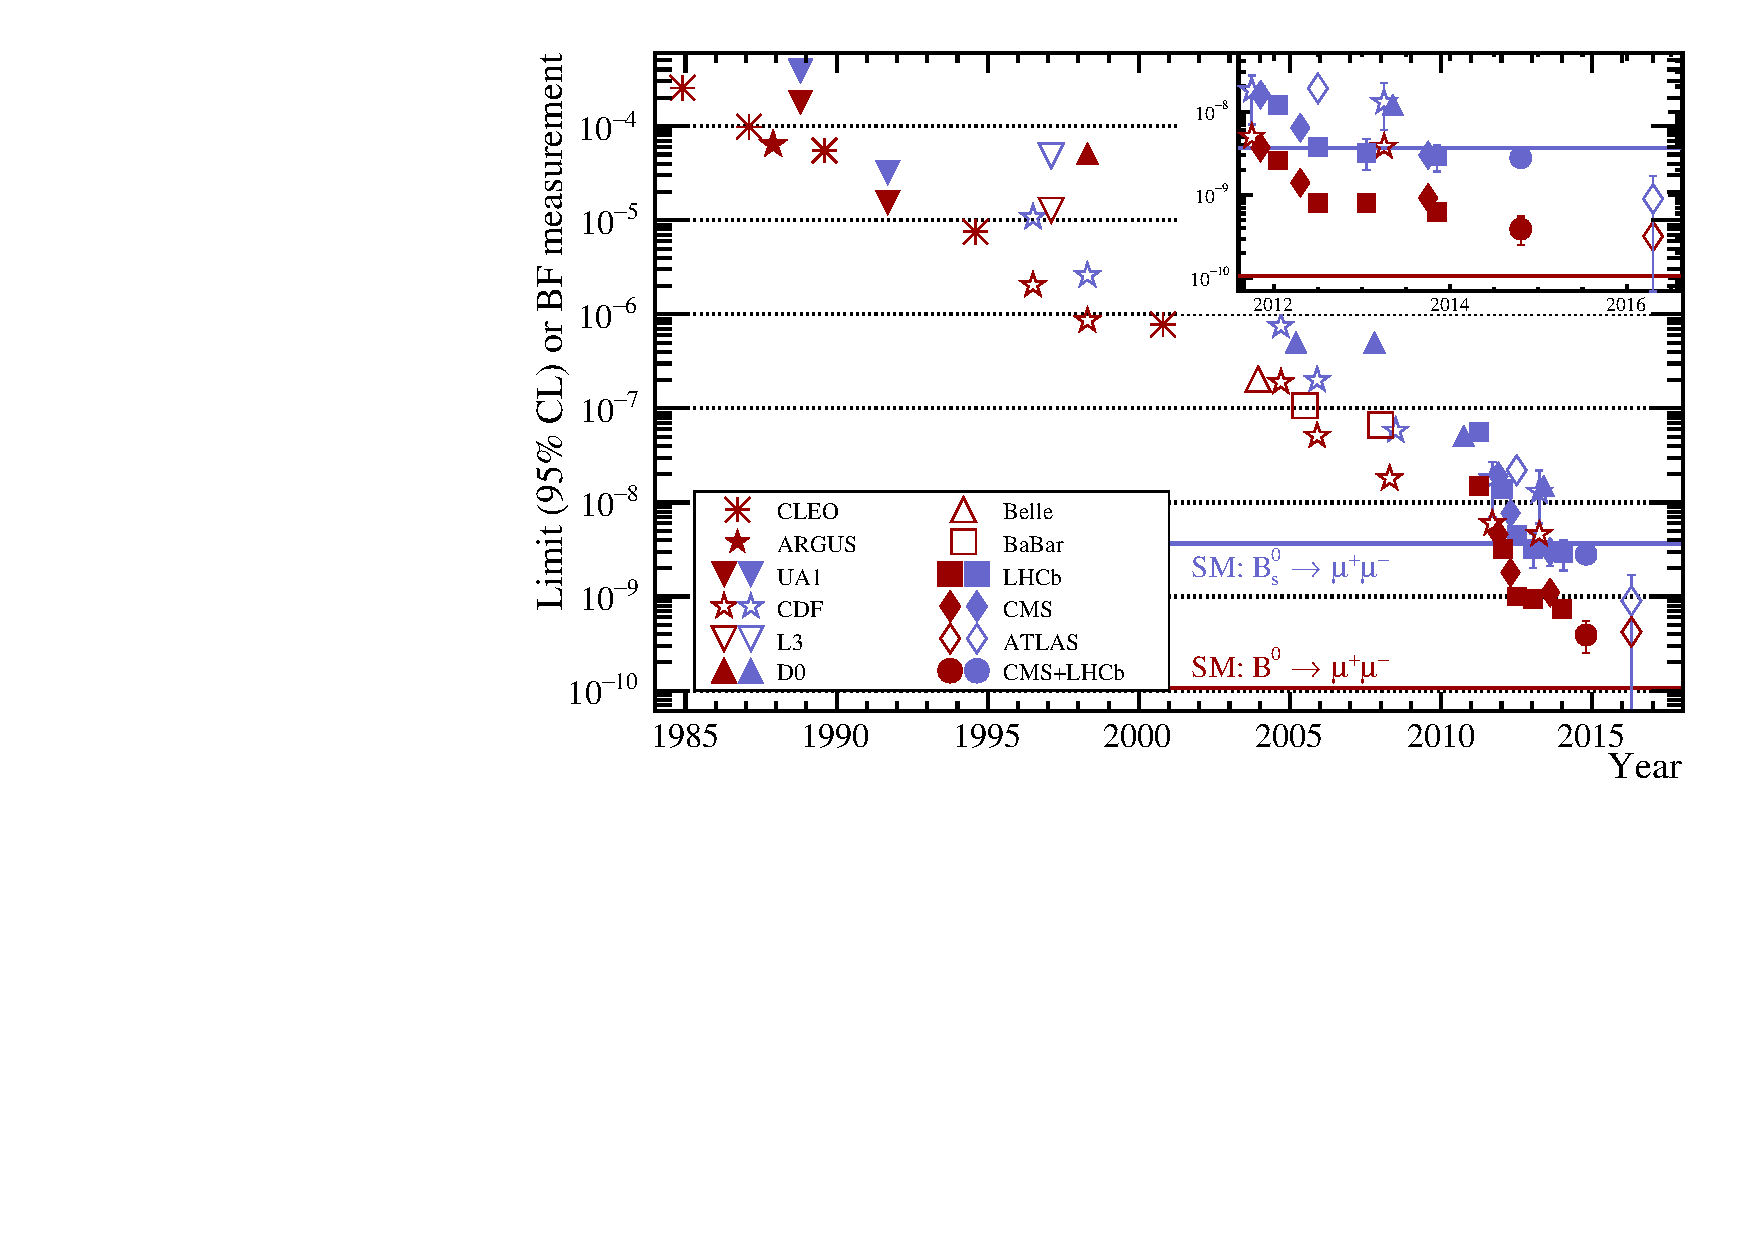
\includegraphics[width=0.8\textwidth]{./Figs/Introduction/95_CL.pdf}
    \caption{Results from searches for \bdmumu (red) and \bsmumu (purple) decays. Upper limits are shown without error bars at the 95$\%$ confidence level. The figure is taken from reference~\cite{CMS:2014xfa} and has been updated to include the latest result from the ATLAS experiment~\cite{Aaboud:2016ire}.}
    \label{fig:bmumu_history}
\end{figure}

The first evidence for \bsmumu decays was found in 2012 by the LHCb experiment~\cite{Aaij:2012nna}. Since then,
the LHCb experiment has measured the \bsmumu \BF to be $\mathcal{B}(B^{0}_{s} \to \mu^+ \mu^-) = (2.9^{+1.1}_{-1.0})\times 10^{-9}$ at a statistical significance of 4.0$\sigma$ and placed a upper limit on the \bdmumu \BF of $\mathcal{B}(B^{0} \to \mu^+ \mu^-) < 7.4 \times 10^{-10}$ at the 95$\%$ confidence level~\cite{Aaij:2013aka}. These measurements were performed using data collected during 2011 and 2012 at the centre-of-mass energies of 7 and 8 TeV, respectively. Searches for \bmumu decays performed by the CMS experiment using data recorded in the same time period corroborated the results from the LHCb experiment. The CMS experiment measured the \bsmumu \BF to be $\mathcal{B}(B^{0}_{s} \to \mu^+ \mu^-) = (3.0^{+1.0}_{-0.9})\times 10^{-9}$ with a statistical significance of 4.3$\sigma$ and placed a limit on the \bdmumu \BF of $\mathcal{B}(B^{0} \to \mu^+ \mu^-) < 1.1 \times 10^{-9}$ at the 95$\%$ confidence level~\cite{Chatrchyan:2013bka}. 
The combined analysis of the CMS and LHCb data sets, collected at centre-of-mass energies of 7 and 8~\tev, resulted in the first observation of \bsmumu decays and the first evidence for \bdmumu decays~\cite{CMS:2014xfa}. The measured branching fractions were 
\begin{equation}
\mathcal{B}(B^{0}_{s} \to \mu^+ \mu^-)_{\mathrm{CMS + LHCb}}  = 2.8^{+0.7}_{-0.6} \times 10^{-9}
\end{equation}
\begin{equation}
\mathcal{B}(B^{0} \to \mu^+ \mu^-)_{\mathrm{CMS + LHCb}}  = 3.9^{+1.6}_{-1.4} \times 10^{-10}
\end{equation}
with a statistical significance of 6.2$\sigma$ for the \bs and 3.0$\sigma$ for the \bd. The ATLAS experiment also searched for \bmumu decay using data collected during the same period~\cite{Aaboud:2016ire}, measuring the \bsmumu \BF as 
\begin{equation}
\mathcal{B}(B^{0}_{s} \to \mu^+ \mu^-)_{\mathrm{ATLAS}}  = 0.9^{+1.1}_{-0.8} \times 10^{-9}
\end{equation}
with a statistical significance of 2.0$\sigma$. An upper limit was placed on the \bdmumu decay of $\mathcal{B}(B^{0}_{s} \to \mu^+ \mu^-) >4.2 \times 10^{-10}$ at the 95 $\%$ confidence level.

Although it was hoped that large deviations from the SM predictions would be found in these decays this has not yet been observed. 
All the measured values are consistent with the expectations of the SM and have enabled constraints to be placed on the parameter space available for New Physics models. Nevertheless, the precision of the measurements allows plenty of room for NP effects to be revealed. Furthermore, there is some tension between the separate measurements themselves and the SM prediction as shown in Figure~\ref{fig:contour}. Therefore, the study of \bmumu decays continues to be a very interesting topic in the search for NP effects. 
 
\begin{figure}[tbp]
    \centering
        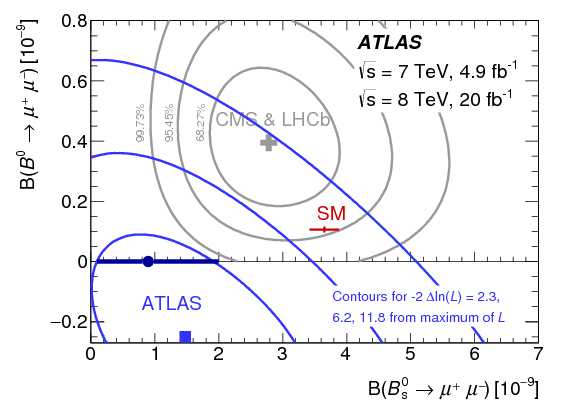
\includegraphics[width=0.7\textwidth]{./Figs/Introduction/contour_plot.png}
        \caption{Measurements of the \bdmumu \BF and \bsmumu \BF from the ATLAS experiment and the combined analysis of CMS and LHCb data alongside the predictions of the SM~\cite{Aaboud:2016ire}. The measurements were performed using data collected during 2011 and 2012 and centre-of-mass energies of 7 and 8~\tev, respectively.}
        \label{fig:contour}
\end{figure}
%The measurements have enabled strong constraints to be placed on the parameter space available for new physics models~\cite{} but the precision of the measurements still allows plenty of room for NP effects to be revealed. 
%Therefore the study of \bmumu decays continues to be an very interesting topic in the search for NP effects. 

%The data collected from $pp$ collisions with centre-of-mass energies of 13 TeV at the LHC will enable more precise measurements of the \BFs of these decays to be made. 
The observation of \bsmumu decays opens the way for other properties of this decay to be studied. In particular the effective lifetime of \bsmumu decays provides a search for NP complementary to the \BF measurement, as the presence of NP could be revealed in either both or only one of these measurements. The search for the \bsmumu decay is complete and the precise study of this decay has begun.
This dissertation documents the latest study of \bmumu decays at the LHCb experiment. Measurements of the \bmumu \BF and the \bsmumu effective lifetime are presented using data collected during $pp$ collisions with centre-of-mass energies of 7, 8 and 13~\tev. %The theoretical motivation for studying these decays is given in Chapter~\ref{sec:theory_chptr} and the LHC and LHCb experiment are described in Chapter~\ref{CERN_LHC_LHCb}. The criteria used to identify these decays in the data are detailed in Chapter~\ref{selection_chapter} and the measurement of the \BF is briefly described in Chapter~\ref{sec:BFanalysis}. The measurement of the \bsmumu effective lifetime is discussed in Chapter~\ref{sec:lifetimemeasurement} and the systematic uncertainties of this measurement are given in Chapter~\ref{sec:systematics}. Finally a summary of the results and prospects for future measurements of \bmumu decays are given in Chapter~\ref{sec:summaryandoutlook}.

